% Kopfzeile beim Kapitelanfang:
\fancypagestyle{plain}{
%Kopfzeile links bzw. innen
\fancyhead[L]{\Large Vorlesung 10 (14.11.2013)}
%Kopfzeile rechts bzw. außen
\fancyhead[R]{}}
%Kopfzeile links bzw. innen
\fancyhead[L]{\Large Vorlesung 10 (14.11.2013)}
%Kopfzeile rechts bzw. außen
\fancyhead[R]{}
% **************************************************
\section{Definition: Betrag einer komplexen Zahl}\label{6.6}
Gegeben sei eine komplexe Zahl $z=x+iy$ ($x,y \in \R$). Der Betrag ist definiert als:
$$|z| := \sqrt{x^2+y^2} = \sqrt{z \overline{z}}$$

\subsection*{Geometrisch (Satz des Pythagoras)}
$|z|$ ist die Länge des Ortsvektors von $z$, bzw. Abstand des Punktes $z$ von $0$.\\
\begin{tikzpicture}
\draw[->](-0.5,0)--(3,0);
\draw[->](0,-0.5)--(0,3);
\draw (-0.3,-0.3) node{$0$};
\draw (1,-0.5) node{$x$};
\draw[->](0,0)--(2,2);
\draw[dashed](2,0)--(2,2);
\draw (2.3,1) node{$y$};
\draw (2.3,2.3) node{$z$};
\draw (0.8,1.3) node{$|z|$};
\end{tikzpicture}

\section{Eigenschaften des Betrags}\label{6.7}
\enk{
\item $|z| \ge 0, |z|=0 \Lra z=0$
\item $|\overline{z}|=|z|$
\item $|\text{Re } z| \le |z|, |\text{Im } z| \le |z|$
\item $|z \cdot w| = |z| \cdot |w|$ \underline{Multiplikativität}
\item $|z+w| \le |z|+|w|$ \underline{Dreiecksungleichung}
\item $||z|-|w|| \le |z-w|$
}

\subsection*{Beweise}
\enk{
\item[4.] $|z \cdot w|^2 = zw \cdot \overline{zw} = z \overline{z} \cdot w \overline{w} = |z|^2 \cdot |w|^2$\\
Wurzelziehen $\Ra |zw| = |z| \cdot |w|$ \qed
\item[5.] $|z+w|^2 = (z+w) \cdot (\overline{z+w}) = (z+w) \cdot (\overline{z} + \overline{w}) = z \overline{z} + (z \overline{w} + \overline{z} w) + w \overline{w} = |z|^2 + 2 \underbrace{\text{ Re} (z \overline{w})}_{\le |z| \cdot |w|} \le (|z|+|w|)^2$ \qed
\item[6.] Folgt aus 5. wie für $\R$ ($z=z-w+w$)
}

\subsection*{Bemerkungen}
\enk{
\item Sei $a \in \C, r > 0 \Ra \{z \in \C: |z-a|=r\}$ Kreis um $a$ mit Radius $r$\\
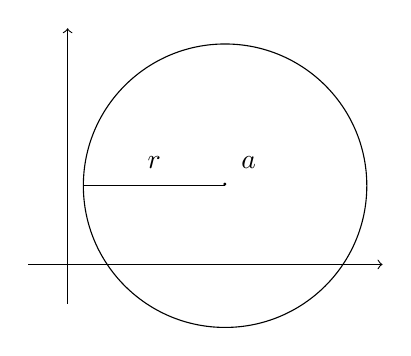
\begin{tikzpicture}
\draw[->](-0.5,0)--(4,0);
\draw[->](0,-0.5)--(0,3);
\draw (2,1) circle (1.8) node{$\cdot$};
\draw (2.3,1.3) node{$a$};
\draw(2,1)--(0.2,1);
\draw (1.1,1.3) node{$r$};
\end{tikzpicture}
\item Zum Invertieren in $\C$:\\
Sei $z=x+iy \in \C, z \neq 0$
$$\Ra \frac{1}{z} \underset{\text{Trick}}{=} \frac{\overline{z}}{z \cdot \overline{z}} = \frac{x-iy}{x^2+y^2} = \frac{x}{x^2+y^2} - i \cdot \frac{y}{x^2+y^2}$$
(wieder in Form $a+ib$)
\item Es gibt keine Anordnung ``$>$'' auf $\C$, bezüglich der $\C$ angeordneter Körper wäre ($\C$ lässt sich nicht anordnen).\\
Denn: Sonst wäre $-1=i^2 > 0 \Ra 1 < 0$, aber $1 > 0$ in jedem angeordneten Körper. \wspruch\\
$z > w, z > 0$ ist im $\C$ nicht sinnvoll; nur die \underline{Beträge} komplexer Zahlen lassen sich der Größe nach vergleichen.
}

\subsection*{Geometrische Interpretation von $+, \cdot$}
\subsubsection*{Addition}
$z=x+iy, w=u+iv \Ra z+w=(x+u)+i(y+v)$\\
Vektoraddition im $\R^2$\\
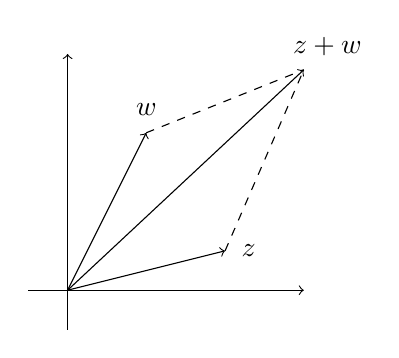
\begin{tikzpicture}
\draw[->](-0.5,0)--(3,0);
\draw[->](0,-0.5)--(0,3);
\draw[->](0,0)--(3,2.8);
\draw(3.3,3.1) node{$z+w$};
\draw[->](0,0)--(2,0.5);
\draw(2.3,0.5) node{$z$};
\draw[->](0,0)--(1,2);
\draw(1,2.3) node{$w$};
\draw[dashed](1,2)--(3,2.8);
\draw[dashed](2,0.5)--(3,2.8);
\end{tikzpicture}

\subsubsection*{Multiplikation}
$z,w \in \C \Ra |zw|=|z| \cdot |w|$\\
Wir werden sehen: $zw$ entsteht aus $z,w$\\
durch Multiplikation der Beträge und Addition der Winkel zur $\R$-Achse.\\
\begin{tikzpicture}
\draw[->](-0.5,0)--(3,0);
\draw[->](0,-0.5)--(0,3);
\draw[->](0,0)--(1.5,0.5);
\draw(1.8,0.5) node{$z$};
\draw[->](0,0)--(0.5,2);
\draw(0.5,2.3) node{$w$};
\draw[->](0,0)--(-0.25,3.25);
\draw(-0.25,3.55) node{$zw$};
\end{tikzpicture}

\subsubsection*{Beispiel}
$z=x+iy=(x,y)$\\
$i \cdot z=-y+ix=(-y,x)$\\
$iz$ entsteht aus $z$ durch Drehung um $90^{\circ}$ gegen den Uhrzeigersinn um $0$.\\
Beachte: $i^4 = (i^2)^2 = (-1)^2 = 1$

\newpage

\phantomsection
\addcontentsline{toc}{section}{\texorpdfstring{Quadratische Gleichungen im $\C$}{Quadratische Gleichungen im \C}}
\section*{Quadratische Gleichungen im $\C$}
Seien $p,q \in \C$. Betrachte die Gleichung:\\
(*) $z^2+pz+q=0$\\
Hat diese Gleichung eine Lösung im $\C$? (*) $\Lra (z+\frac{p}{2})^2 = -1+\frac{p^2}{4} =: c$\nl
Sei $c=a+ib \in \C$ ($a,b \in \R$)\\
Gesucht ist: $z \in \C$ mit $z^2=c$.\\
Mit $z$ ist dann auch $-z$ Lösung.\nl
Ansatz: $z=x+iy$ ($x,y \in \R$)\\
$z^2 = c \Lra (x+iy)^2 = a+ib \Lra x^2+2ixy-y^2 = a+ib \underset{\text{Vergleich der Re- und Im-Teile}}{\Lra} x^2-y^2=a \wedge 2xy = b$\nl
Beachte: Zwei komplexe Zahlen sind genau dann gleich, wenn ihre Re- und Im-Teile gleich sind.\\
Auflösen nach $x,y$ liefert zwei komplexe Lösungen $z_1=x_1+iy_1, z_2=-z_1$\\
Schreibe: $z_{1/2} = \pm \sqrt{c}$ (Randfall: $x=0 \Ra z_1=z_2=0$)\\
Damit: (*) hat die Lösungen $z_{1/2} = - \frac{p}{2} \pm \sqrt{\frac{p^2}{4} - q}$

\phantomsection
\addcontentsline{toc}{section}{\texorpdfstring{Algebraische Gleichungen im $\C$}{Algebraische Gleichungen im \C}}
\section*{Algebraische Gleichungen im $\C$}
Eine algebraische Gleichung in $\C$ ist eine Gleichung der Form
$$z^n + a_{n-1}z^{n-1}+ \ldots +za_1+a_0=0$$
mit Koeffizienten $a_0,\ldots,a_{n-1} \in \C, n \in \N$ und unbekanntem $z \in \C$.

\section{Satz: Fundamentalsatz der Algebra}\label{6.8}
Jede algebraische Gleichung hat mindestens eine Lösung im $\C$.

\subsection*{Beweis}
Ausgelassen

\subsection*{Vorbemerkung: Algebraische Operationen mit Funktionen}
\emph{Hier: $\K$ einer der Körper $\R$ oder $\C$.}\nl
Seien $f,g: X \to \K$ Funktionen ($X$ Menge, z.B. $\R, \C$)\\
Definiere $f \pm g, f \cdot g: X \to \K$ so:
$$(f \pm g)(x) := f(x) \pm g(x)$$
$$(f \cdot g)(x) := f(x) \cdot g(x)$$

\subsection*{Beispiel}
$f,g: \C \to \C, f(z) = z^2, g(z)=z^3 \Ra (f \cdot g)(x)=z^5$\\
Ferner: $\frac{f}{g}: \{x \in X: g(x) \neq 0\} \to \K, \bigbrackets{\frac{f}{g}}(x) := \frac{f(x)}{g(x)}$

\section{Definition: Polynome}\label{6.9}
Eine Funktion $p: \K \to \K$ (mit $\K = \R \vee \C$) der Form
$$p(x) = a_n x^n + a_{n-1} x^{n-1} + \ldots + a_1 x + a_0$$
mit $n \in \N_0$, $a_0,\ldots,a_n \in \K$ heißt \underline{Polynomfunktion (kurz: Polynom) über $\K$}.\\
$a_j$ sind die Koeffizienten von $p$.\\
Ist $a_n \neq 0$, so heißt $n$ der \underline{Grad von p}, $n=\text{grad }p$.\\
Sind alle $a_j = 0$, so heißt $p$ das Nullpolynom ($p=0$).
$$\text{grad }0 := -\infty$$
$$\Pow_\K := \{p: \K \to \K: p \text{ Polynom}\}$$
Summen und Produkte von Polynomen sind wieder Polynome.\\
Etwa: $p(x) = a_n x^n + \ldots + a_1 x + a_0$ und $q(x) = b_m x^m + \ldots + b_1 x + b_0$\\
$\Ra (pq)(x) = c_{n+m} x^{n+m} + \ldots + c_ x + c_0$\\
mit $c_{n+m} = a_n b_m$, $c_0 = a_0 b_0$ $c_1 = a_1 b_0 + a_0 b_1$, $c_2 = a_2 b_0 + a_1 b_1 + a_2 b_2$\\
allgemein: $c_k = \sum_{j=0}^k a_j b_{k-j}$

\section{Polynomdivision mit Rest}\label{6.10}
Seien $p,q \in \Pow_\K$, $q \neq 0$\\
$\Ra$ es gibt eindeutige $r,s \in \Pow_\K$ mit $p=sq+r$, wobei $\text{grad }r < \text{grad }q$ ($-\infty < n \forall n \in \N_0$)

\subsection*{Beweis}
Ausgelassen

\subsection*{Beispiel}
$p(x)=x^3+2x^2-3x+4$, $q(x)=x^2+1$\\
\polyset{style=C, div=:,vars=x}
\polylongdiv{x^3+2x^2-3x+4}{x^2+1}\\
$-4x+2=r(x)$ ist der Rest.

\subsection*{Bezeichnung}
\items{
\item Ist $r=0$ in \ref{6.10}, das heißt $p=sq$, so heißt $q$ ein Teiler von $p$.
\item $\alpha \in \K$ heißt \underline{Nullstelle} von $p \in \Pow_\K$, falls $p(x)=0$
}

\section{Korollar: Abspalten von Linearfaktoren zur Nullstelle}\label{6.11}
Sei $p(\alpha)=0 \Ra \exists! s \in \Pow_\K: p(x)=(x-\alpha) \cdot s(x)$.\\
Dabei ist $\text{grad }s = \text{grad }p -1$